% Unofficial University of Cambridge Poster Template
% https://github.com/andiac/gemini-cam
% a fork of https://github.com/anishathalye/gemini
% also refer to https://github.com/k4rtik/uchicago-poster

\documentclass[final]{beamer}

% ====================
% Packages
% ====================

\usepackage[T1]{fontenc}
\usepackage{lmodern}
\usepackage[orientation=portrait,size=a0,scale=1.0]{beamerposter}
\usetheme{gemini}
\usecolortheme{nott}
\usepackage{graphicx}
\graphicspath{{figures/}}
\usepackage{float}
\usepackage{subfloat}
\usepackage{caption}
\usepackage{subcaption}
\usepackage{wrapfig}
\usepackage{booktabs}
\usepackage{tikz}
\usetikzlibrary{bayesnet}
\usetikzlibrary{arrows}
\usepackage{pgfplots}
\pgfplotsset{compat=1.18}
\usepackage{anyfontsize}
\usepackage{multirow}
\usepackage{stmaryrd}
\usepackage{algorithm}
\usepackage[noend]{algpseudocode}
\usepackage{amsmath}
\usepackage{multicol}

\setbeamertemplate{bibliography entry article}{}
\setbeamertemplate{bibliography entry title}{}
\setbeamertemplate{bibliography entry location}{}
\setbeamertemplate{bibliography entry note}{}

% ====================
% Lengths
% ====================

\newlength{\sepwidth}
\newlength{\colwidth}
\setlength{\sepwidth}{0.015\paperwidth}
\setlength{\colwidth}{0.46\paperwidth}

% ====================
% Macros
% ====================

\newcommand{\fracpartial}[2]{\frac{\partial #1}{\partial  #2}}
\newcommand{\prob}{\mathbb{P}}
\newcommand{\R}{\mathbb{R}}
\newcommand{\N}{\mathbb{N}}
\newcommand{\E}{\mathbb{E}}
\renewcommand{\O}{\mathcal{O}}
\renewcommand{\L}{\mathcal{L}}
\newcommand{\eps}{\varepsilon}
\newcommand{\dd}{\, \mathrm{d}}
\newcommand{\J}{\mathcal{J}}
\DeclareMathOperator*{\argmin}{arg\,min}
\DeclareMathOperator*{\argmax}{arg\,max}
\DeclareMathOperator*{\minimize}{minimize}
\DeclareMathOperator*{\KL}{KL}
\newcommand{\intset}[2]{\{#1, ..., #2\}}
\newcommand{\mnbs}{\nobreak\hspace{.16667em}}
\newcommand{\jump}{\newline\newline}
\newcommand{\separatorcolumn}{\begin{column}{\sepwidth}\end{column}}

% ====================
% Header, footer, etc.
% ====================

\title{Mixture Models for Graph Clustering}

\author{Sofiane Ezzehi \inst{1} \and Bastien Le Chenadec \inst{1} \and Theïlo Terrisse \inst{1}}

\institute[shortinst]{École des Ponts ParisTech}

\footercontent{
  \href{https://github.com/bastienlc/mmrg}{https://github.com/bastienlc/mmrg} \hfill Probabilistic Graphical Models
   \hfill
  Master Mathématiques Vision Apprentissage}

\logoright{
\includegraphics[height=4cm]{figures/logo_mva.png}}
\logoleft{
\includegraphics[height=4cm]{figures/logo_ens.png}}

% ====================
% Body
% ====================

\begin{document}

\begin{frame}[t]
  \begin{columns}[t]
    \separatorcolumn

    \begin{column}{\colwidth}

      \begin{block}{Graph Clustering}


        \textbf{Graph clustering} involves the identification of clusters within a graph, where nodes exhibit denser connections among themselves than with the rest of the network. This task is crucial for conducting comprehensive macro- and mesoscopic analyses of large complex systems, such as social networks. As exact graph clustering is recognized as an NP-hard problem, numerous clustering methods have been developed \cite{fortunato_community_2010}. Notably, model-based approaches fit a mathematical model to a graph, providing an explanatory framework for observed connectivity patterns. In \cite{main_article}, J.-J. Daudin \textit{et al.} investigate the renowned \textbf{Stochastic Block Model (SBM)}, proposing a \textbf{variational Expectation-Maximization (EM)} algorithm to optimize model fit for a given graph.
      \end{block}

      \begin{block}{The Stochastic Block Model}
        \begin{column}{0.5\colwidth}
          \justifying
          \textbf{Stochastic Block Model}: A \textit{mixture} model for graphs where each node is assigned to a \textit{class} and the edge probability between nodes are conditioned on their class memberships. %This model draws inspiration from mixture models for distribution of degrees, and the Erdös-Rényi model which deals with the probability for two given nodes of being connected.
          \newline\newline
          \textbf{Formally,} let $\mathcal{G}$ be an undirected graph with $n$ nodes and no self-loop, and $X$ its adjacency matrix, \textit{i.e.} $X_{ij} = 1$ if an edge exists between $i$ and $j$, and $X_{ij} = 0$ otherwise.
        \end{column}
        \begin{column}{0.5\colwidth}
          \begin{figure}[H]
            \centering
            \tikz{
              \node[obs] (X_{ij}) {\normalsize $X_{ij}$};
              \node[latent,left=of X_{ij}, xshift=-3cm, label={[name=label1,text height=0.8em]below:$i=1,\dots,n$}] (Z_i) {\large $Z_i$};
              \node[latent,right=of X_{ij}, xshift=3cm, label={[name=label2,text height=0.8em]below:$j=i+1,\dots,n$}] (Z_j) {\large $Z_j$};
              \node[const, above=of X_{ij}, yshift=0cm](alpha){\large $\alpha$};
              \node[const, below=of X_{ij}, yshift=-1.6cm](pi){\large  $\pi$};
              \plate [inner sep=.5cm] {} {(Z_i)(X_{ij})(Z_j)(label1)(label2)} {};
              \plate [inner sep=.25cm] {} {(Z_j)(X_{ij})(label2)} {};
              \edge {Z_i,Z_j} {X_{ij}}
              \edge {alpha} {Z_i}
              \edge {alpha} {Z_j}
              \edge {pi} {X_{ij}}
            }
            \caption{Graphical model of the SBM}
            \label{fig:graphical_model}
          \end{figure}
        \end{column}

        The model is parametrized by $Q$ the number of classes, $\alpha\in [0,1]^Q$ the prior distribution on the classes, and $\pi\in [0,1]^{Q\times Q}$ the probability of an edge between two nodes of different classes. We also introduce the random variables $Z_i\in \{0,1\}^Q$ for $i\in \llbracket 1,n \rrbracket$, that represent the membership of node $i$ to each class. The prior distributions on $Z$ and $X$ are given by :
        \begin{equation*}
          \begin{cases}
            \forall i\in \llbracket 1,n \rrbracket, \quad \sum_{q=1}^Q Z_{iq} = 1 \quad\text{(unique class)}            \\
            \forall q\in \llbracket 1,Q \rrbracket,\quad \mathbb{P}(Z_{iq}=1)=\alpha_q \quad\text{(class distribution)} \\
            \forall q,l\in \llbracket 1,Q \rrbracket, \quad \forall i\neq j\in \llbracket 1,n \rrbracket, \quad \mathbb{P}(X_{ij}=1\,|\,Z_{iq}=1,Z_{jl}=1)=\pi_{ql} \quad\text{(edge probability)}
          \end{cases}
        \end{equation*}
      \end{block}

      \begin{alertblock}{The variational Expectation-Maximization algorithm}
        In \cite{main_article}, Daudin \textit{et al.} propose a variational EM algorithm to fit the SBM.
        \begin{equation*}
          \log \mathcal{L}(X, Z) =  \sum_{i}\sum_{q} Z_{iq}\log\alpha_q + \frac{1}{2}\sum_{i\neq j}\sum_{q,l} Z_{iq}Z_{jl} \, \log\left( \pi_{ql}^{X_{ij}}\left(1-\pi_{ql}\right)^{1-X_{ij}} \right)
        \end{equation*}
        $\implies$ No closed-form solution for the parameters of the model from the likelihood.
        \newline
        \textbf{Problem :} Using an EM algorithm, no closed-form solution for the E-step either. %! 
        \newline
        \textbf{Solution:} Daudin \textit{et al.} search for an approximated distribution $R_X$ of $Z$ given $X$, among the family of product of multinomial distributions, thus introducing the random variables $\tau_i\in [0,1]^Q$ for $i\in \llbracket 1,n \rrbracket$. This approximation leads to maximizing the following lower bound of $\log \mathcal{L}(X)$ :
        \begin{equation*}
          \label{eq:lower_bound}
          \mathcal{J}(R_X)=\log \mathcal{L}(X)-\KL[R_X(\cdot), P(\cdot|X)]
        \end{equation*}
        The authors derive a closed form solution for the M-step, and a \textbf{fixed-point relation} for the E-step :
        \begin{equation*}
          \begin{cases}
            \text{(E-step)} \quad & \hat{\tau}_{iq}\propto \alpha_q \prod_{j\neq i}\prod_l \left[\pi_{ql}^{X_{ij}}(1-\pi_{ql})^{1-X_{ij}}\right]^{\hat{\tau}_{jl}}                                         \\
            \text{(M-step)} \quad & \hat{\alpha}_q=\frac{1}{n}\sum_{i} \tau_{iq} \quad \text{ and } \quad \hat{\pi}_{ql}=\frac{\sum_{i\neq j} \tau_{iq}\tau_{jl}X_{ij}}{\sum_{i\neq j} \tau_{iq}\tau_{jl}}
          \end{cases}
        \end{equation*}
        \centering
        \begin{minipage}{.9\linewidth}
          \begin{algorithm}[H]
            \caption{Variational Expectation-Maximization Algorithm}
            \label{alg:Daudin-EM}
            \begin{algorithmic}[1]
              \State \textbf{Input:} Adjacency matrix $X$, number of communities $Q$
              \State \textbf{Initialize:} Initialize $\tau_{iq}$ for $i \in \llbracket 1, n \rrbracket$, $q \in \llbracket 1, Q \rrbracket$
              \While{not converged}
              \State \textbf{\emph{E-step:}}
              \For{$i \in \llbracket 1, n \rrbracket$}
              \For{$q \in \llbracket 1, Q \rrbracket$}
              \State \textbf{\emph{Fixed-point algorithm:}}
              \State $\hat{\tau}_{iq} \propto \alpha_q \prod_{j\neq i}\prod_l \left[\pi_{ql}^{X_{ij}}(1-\pi_{ql})^{1-X_{ij}}\right]^{\hat{\tau}_{jl}}$\Comment{Update class memberships}
              \EndFor
              \EndFor
              % \State
              \State \textbf{\emph{M-step:}}
              \For{$q \in \llbracket 1, Q \rrbracket$}
              \State $\hat{\alpha}_q = \frac{1}{n}\sum_{i} \tau_{iq}$ \Comment{Update class proportions}
              \State $\hat{\pi}_{ql} = \frac{\sum_{i\neq j} \tau_{iq}\tau_{jl}X_{ij}}{\sum_{i\neq j} \tau_{iq}\tau_{jl}}$ \Comment{Update edge probabilities}
              \EndFor
              \EndWhile
              \State \textbf{Return:} $\hat{\alpha}, \hat{\pi}, \hat{\tau}$
            \end{algorithmic}
          \end{algorithm}
        \end{minipage}

      \end{alertblock}

      \begin{block}{Some alternative algorithms}
        \begin{itemize}
          \item \justifying \textbf{Newman \textit{et al.} \cite{newman}} use a finer definition for clusters. While Daudin \textit{et al.} define a cluster-cluster affinity (nodes belonging to the same cluster behave the same way), the model of Newman introduces a cluster-node affinity. Therefore, edges between different nodes of the same two clusters are not necessarily equivalent. $\implies$ $\Pi_{q,i}$ denotes the probability of an edge between a node in cluster $q$ and node $i$.

                The expected log-likelihood (with respect to $Z$) is
                \begin{equation*}
                  \mathcal{L}(X) = \sum_{i=1}^n\sum_{q=1}^Q \tau_{iq} \left[ \log(\alpha_q) + \sum_{j=1}^n X_{ij} \log(\Pi_{q, j}) \right] \quad \text{where} \quad \tau_{iq} = \mathbb{P}(Z_{iq} = 1 | X, \alpha, \Pi).
                \end{equation*}

                Denoting $k_i$ he degree of node $i \in \llbracket 1, n \rrbracket$, the EM updates are
                \begin{equation*}
                  \text{(E-step) }\,\hat{\tau}_{iq} = \frac{\alpha_q\prod_{j=1}^N \Pi_{qj}^{X_{ij}}}{\sum_{s=1}^Q \alpha_s\prod_{j=1}^N \Pi_{sj}^{X_{ij}}}; \qquad \text{(M-step) }\,\hat{\alpha}_q = \frac{1}{n} \sum_{i=1}^n \tau_{iq} \,\text{ and }\, \hat{\Pi}_{qj} = \frac{\sum_{i=1}^n X_{ij}\tau_{iq} }{\sum_{i=1}^n k_i \tau_{iq}}
                \end{equation*}
                The update of $\tau$ (E-step) is now \textbf{deterministic}, with no resort to fixed-point methods.

          \item \textbf{Spectral clustering \cite{spectral}} uses the eigenvectors of the Laplacian matrix of the graph to cluster the nodes. The $k$ first eigenvectors of $L = D - X$ are stacked in a matrix $U \in \mathbb{R}^{n \times k}$ and a $k$-means clustering is performed on the rows of $U$.
        \end{itemize}
      \end{block}

      \begin{block}{References}
        % \mbox{}\vspace{-1\baselineskip}
        \footnotesize{\bibliographystyle{plain}\bibliography{poster}}
      \end{block}

    \end{column}

    \separatorcolumn

    \begin{column}{\colwidth}

      \begin{block}{Experiments: SBM dataset}
        \begin{column}{0.3\colwidth}
          \justifying
          % \usebeamertemplate{itemize item}
          \textbf{Algorithm \ref{alg:Daudin-EM}} is implemented in PyTorch.
          To test it, a first dataset is created by sampling the SBM for parameters given in \textbf{Table \ref{tab:sbm_parameters}}. For each experiment, 10 graphs are generated and the algorithm is run for $100$ iterations on each graph.\\[0.5em]
          \textbf{Figure \ref{fig:sbm_exp}} shows the results.
        \end{column}
        \begin{column}{0.7\colwidth}
          \begin{table}[ht]
            \centering
            \small
            \setlength\heavyrulewidth{0.25ex}
            \begin{tabular}{@{}cccccc@{}}
              \toprule
              \multicolumn{2}{c}{\textbf{Experiment}} & \multicolumn{2}{c}{\textbf{Hyper-parameters}} & \multicolumn{2}{c}{\textbf{Parameters}}                                                                                                                                      \\
              \#                                      & Name                                          & \hspace{1em} $n$                        & $Q$                    & $\alpha$                                  & $\pi$                                                         \\ \midrule \midrule
              1                                       & \multicolumn{1}{c|}{Random}                   & \hspace{1em} 500                        & \multicolumn{1}{c|}{3} & $\alpha \sim \text{Dir}(1.5)$             & $\pi_{ij} \sim \mathcal{U}([0, 1))$                           \\
              2                                       & \multicolumn{1}{c|}{Homophilic}               & \hspace{1em} 150                        & \multicolumn{1}{c|}{5} & $\alpha_i = (\frac{1}{Q})_i$              & $\pi_{ii} \sim \mathcal{U}([0.5, 1)), \ \pi_{ij} = 0.01$      \\
              3                                       & \multicolumn{1}{c|}{Heterophilic}             & \hspace{1em} 150                        & \multicolumn{1}{c|}{3} & $\alpha_i = (\frac{1}{Q})_i$              & $\pi_{ii} = 0.01, \ \pi_{ij} = 0.9$                           \\
              4                                       & \multicolumn{1}{c|}{Dense minority}           & \hspace{1em} 150                        & \multicolumn{1}{c|}{2} & $\alpha^T = (\frac{9}{10}, \frac{1}{10})$ & $\pi = \begin{pmatrix} 0.01 & 0.7 \\ 0.7 & 0.8 \end{pmatrix}$ \\ \bottomrule
            \end{tabular}
            \caption{\centering Parameters for generating the SBM dataset. \\ $\text{Dir}$ is the Dirichlet law. In experiment 1, $\pi$ is scaled and made symmetric.}
            \label{tab:sbm_parameters}
          \end{table}
        \end{column}
        % \usebeamertemplate{itemize item} 
        %For each experiment, a sample graph is visualized (with one color per cluster) along with the prediction.
        \textcolor{nottblue}{\usebeamertemplate{itemize item}}
        \textbf{Metric for model-fitting capacity}: Sum of (cluster-permutation-invariant) Euclidean distances between predicted $(\alpha, \pi)$ and the ground truth of Table \ref{tab:sbm_parameters}. The result is normalized by the number of classes.
        \newline
        \textcolor{nottblue}{\usebeamertemplate{itemize item}}
        \textbf{Metric for clustering capacity}: Normalized Mutual information (NMI) and Rand Index (RI).\newline
        \textbf{NB}: The fixed-point algorithm does not always converge within $1000$ iterations for all graphs.

        \begin{figure}[h]
          \begin{subfigure}{0.49\linewidth}
            \centering
            % \hfill
            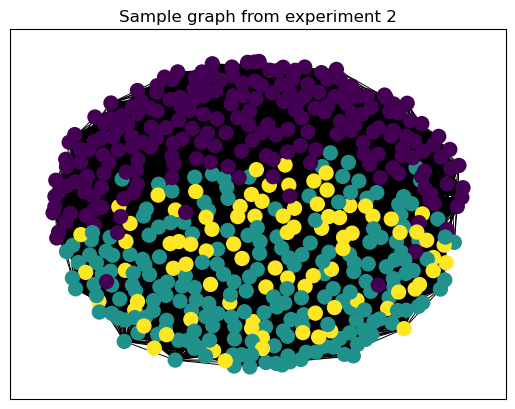
\includegraphics[width=0.49\linewidth, trim={5 5 5 18}, clip]{figures/exp2_sample.png}
            % \hfill
            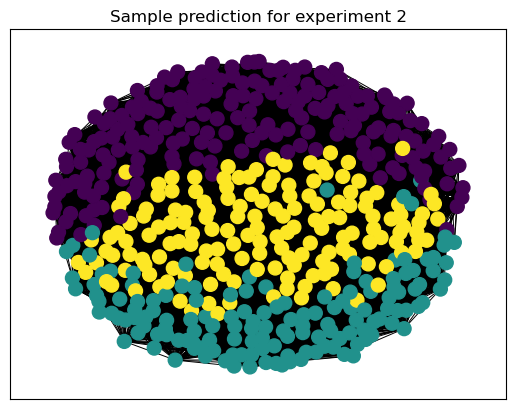
\includegraphics[width=0.49\linewidth, trim={5 5 5 18}, clip]{figures/exp2_pred.png}
            % \hfill
            \caption{\centering Experiment 1: 8/10 graphs passed\\ $\mathrm{Param. dist.} = 0.08 \pm 0.03, \ \mathrm{NMI} = 0.33 \pm 0.13, \ \mathrm{RI} = 0.66 \pm 0.13$}
            \label{fig:exp1}
          \end{subfigure}
          \hfill
          \begin{subfigure}{0.49\linewidth}
            \centering
            % \hfill
            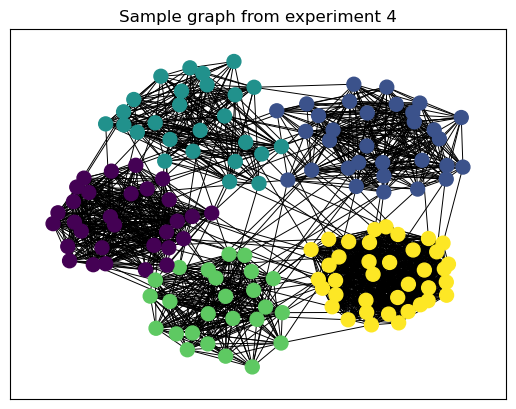
\includegraphics[width=0.49\linewidth, trim={5 5 5 18}, clip]{figures/exp4_sample.png}
            % \hfill
            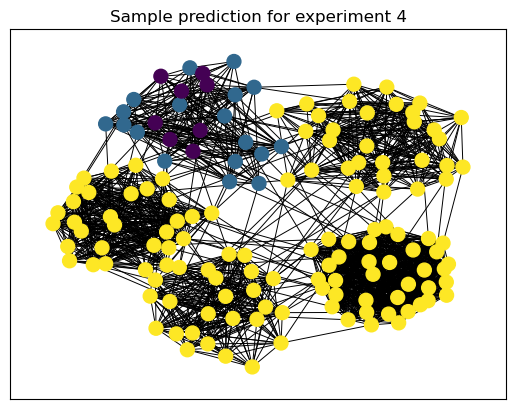
\includegraphics[width=0.49\linewidth, trim={5 5 5 18}, clip]{figures/exp4_pred.png}
            % \hfill
            \caption{\centering Experiment 2: 4/10 graphs passed\\ $\mathrm{Param. dist.} = 0.22 \pm 0.02, \ \mathrm{NMI} = 0.11 \pm 0.18, \ \mathrm{RI} = 0.27 \pm 0.12$}
            \label{fig:exp2}
          \end{subfigure}
          \medskip
          \begin{subfigure}{0.49\linewidth}
            \centering
            % \hfill
            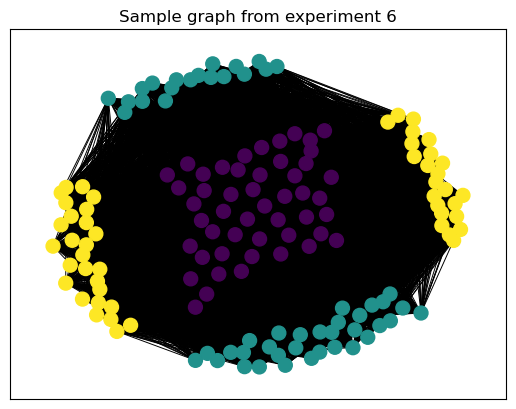
\includegraphics[width=0.49\linewidth, trim={5 5 5 18}, clip]{figures/exp6_sample.png}
            % \hfill
            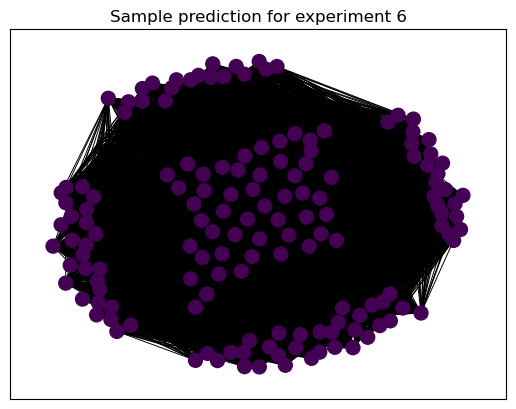
\includegraphics[width=0.49\linewidth, trim={5 5 5 18}, clip]{figures/exp6_pred.png}
            % \hfill
            \caption{\centering Experiment 3: 9/10 graphs passed\\ $\mathrm{Param. dist.} = 0.18 \pm 0.08, \ \mathrm{NMI} = 0 \pm 0, \ \mathrm{RI} = 0.33 \pm 0$}
            \label{fig:exp3}
          \end{subfigure}
          \hfill
          \begin{subfigure}{0.49\linewidth}
            \centering
            % \hfill
            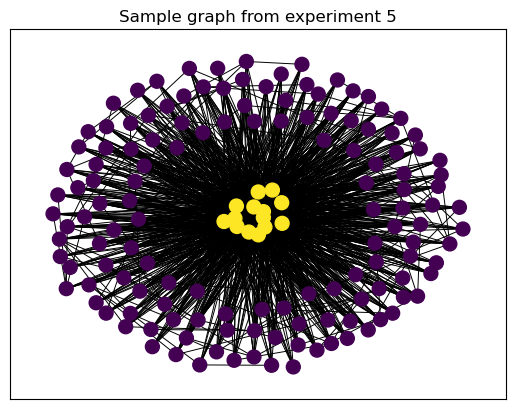
\includegraphics[width=0.49\linewidth, trim={5 5 5 18}, clip]{figures/exp5_sample.png}
            % \hfill
            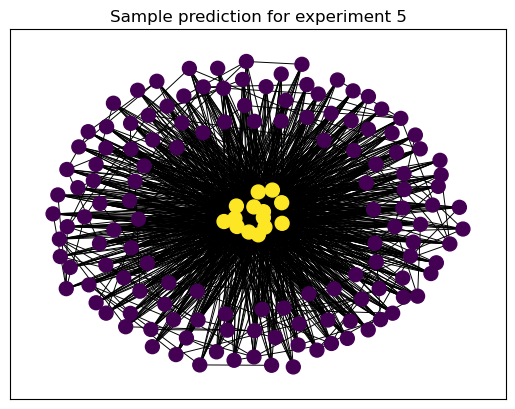
\includegraphics[width=0.49\linewidth, trim={5 5 5 18}, clip]{figures/exp5_pred.png}
            % \hfill
            \caption{\centering Experiment 4: 10/10 graphs passed\\ $\mathrm{Param. dist.} = 0.02 \pm 0.01, \ \mathrm{NMI} = 1 \pm 0, \ \mathrm{RI} = 1 \pm 0$}
            \label{fig:exp4}
          \end{subfigure}
          \caption{Results for the SBM dataset experiments. Left: sample graph; right: associated prediction.}
          \label{fig:sbm_exp}
        \end{figure}
      \end{block}

      \begin{block}{Experiments: Cora dataset}
        All three methods are tested on the \textbf{Cora citation network} \cite{cora}: an undirected graph of 2708 nodes (\textit{i.e.}, scientific papers) connected by 5429 edges (\textit{i.e.}, citations). Nodes are labeled into 7 different classes:\\
        {\small \centering \textbf{1:} Cases $-$ \textbf{2:} Genetic Alg. $-$ \textbf{3:} Neural Net. $-$ \textbf{4:} Prob. Methods $-$ \textbf{5:} Reinforcement Learning $-$ \textbf{6:} Rule Learning $-$ \textbf{7:} Theory}
        \begin{column}{0.73\colwidth}
          \begin{figure}[H]
            \centering
            \hfill
            \begin{subfigure}{0.45\linewidth}
              \centering
              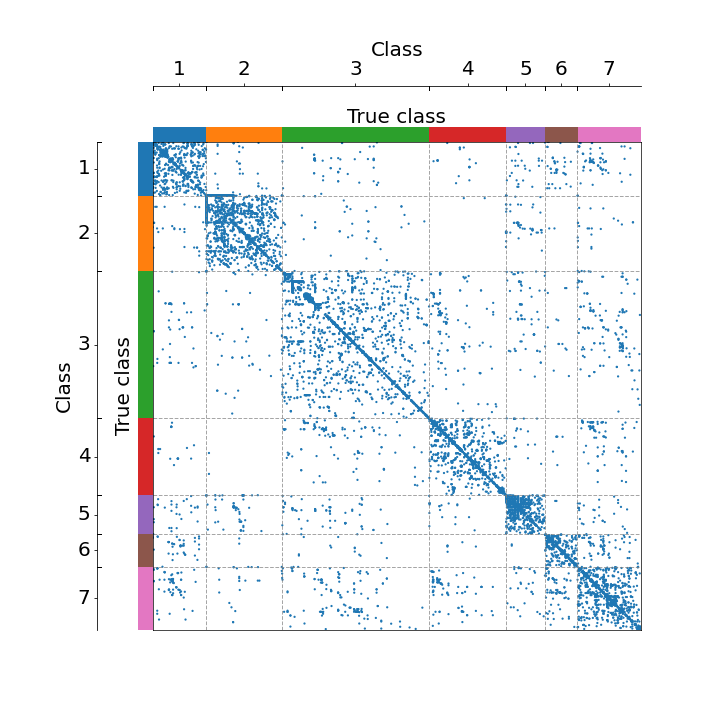
\includegraphics[width=\linewidth, trim={45 25 35 40}, clip]{figures/cora_gt.png}
              \caption{Ground truth
              }
              \label{fig:cora_gt}
            \end{subfigure}
            \hspace{0.5em}
            \begin{subfigure}{0.45\linewidth}
              \centering
              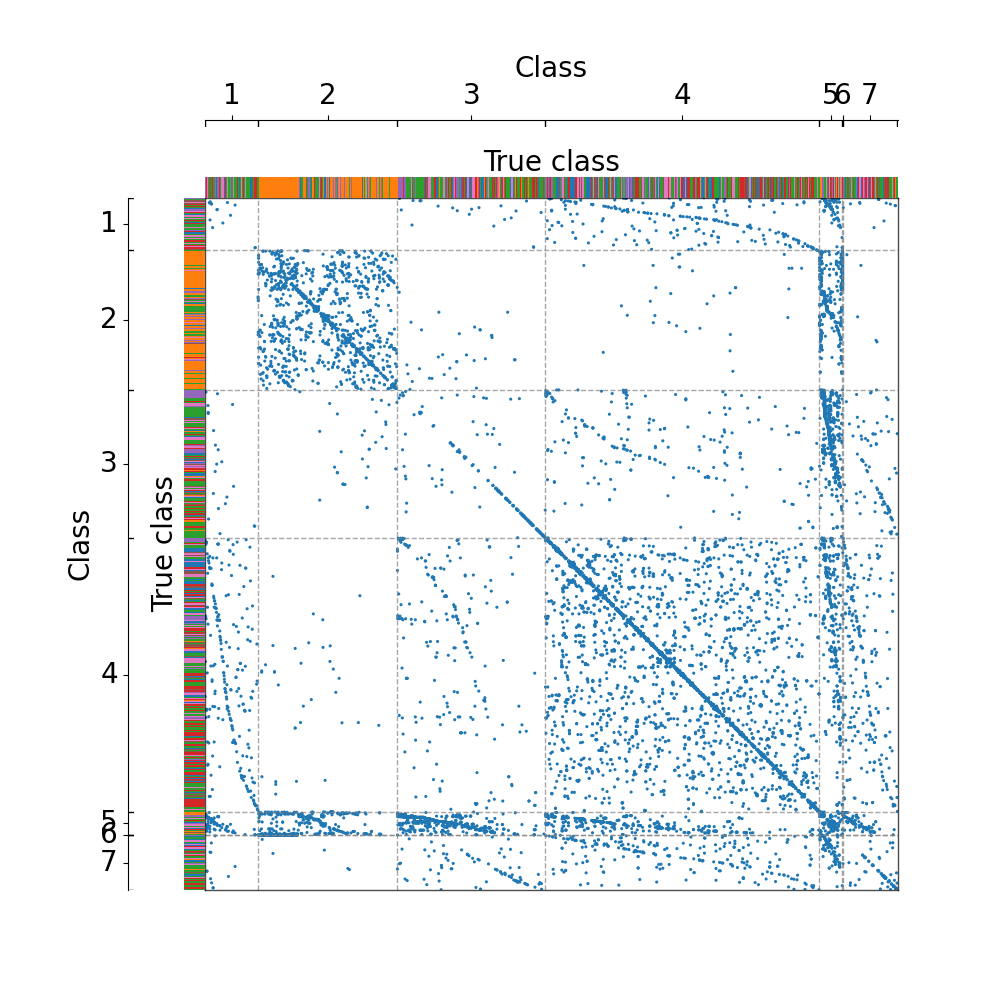
\includegraphics[width=\linewidth, trim={45 25 35 40}, clip]{figures/cora_sbm.png}
              \caption{Daudin \textit{et al.} (50 iterations)}
              \label{fig:cora_SBM}
            \end{subfigure}
            \hfill
            \medskip
            \hfill
            \begin{subfigure}{0.45\linewidth}
              \centering
              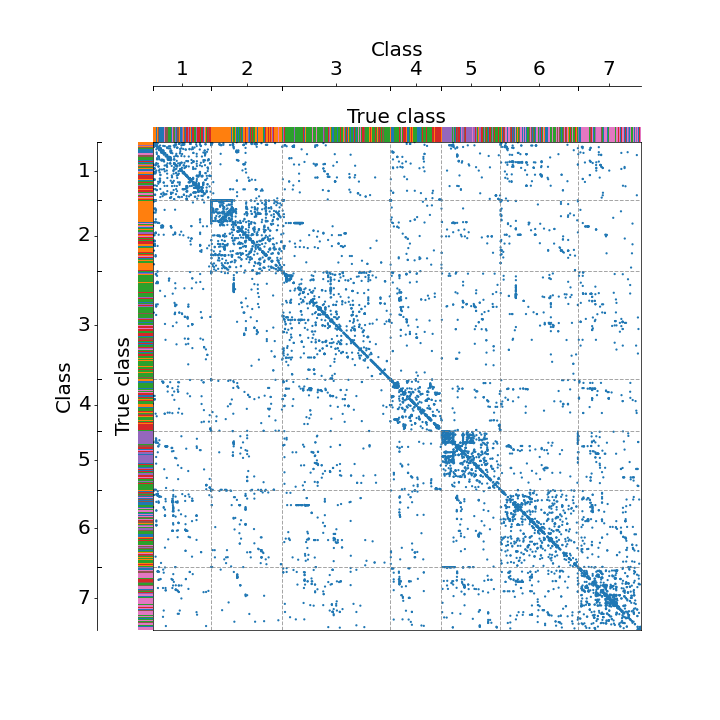
\includegraphics[width=\linewidth, trim={45 25 35 40}, clip]{figures/cora_Newman.png}
              \caption{Newman \textit{et al.} (100 iterations)}
              \label{fig:cora_newman}
            \end{subfigure}
            \hspace{0.5em}
            \begin{subfigure}{0.45\linewidth}
              \centering
              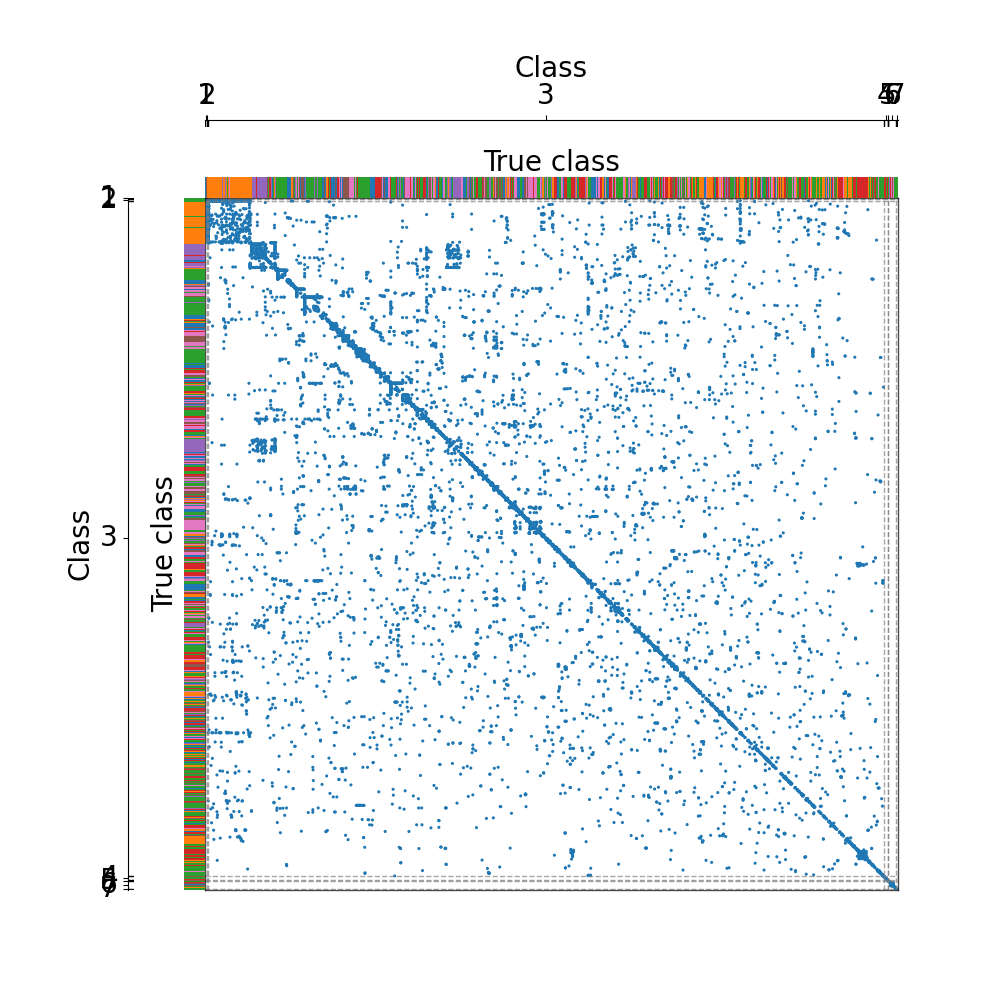
\includegraphics[width=\linewidth, trim={45 25 35 40}, clip]{figures/cora_spetral.png}
              \caption{Spectral clustering}
              \label{fig:cora_spectral}
            \end{subfigure}
            \hfill
            \caption{\centering Dot-plot of the clustering of Cora for all $3$ methods}
            \label{fig:cora_results}
          \end{figure}
        \end{column}
        \begin{column}{0.27\colwidth}
          \vspace{4em}
          \begin{itemize} \setlength\itemsep{1.5em}
            \justifying
            \item \textbf{Daudin-EM} yields similar results as \textbf{Newman-EM} for the supervised metrics.
            \item \textbf{Daudin-EM} reveals some good-quality clusters (2, 4) despite some clusters having a clustering coefficient of 0.
            \item \textbf{Newman-EM} predicts the closest clustering coefficients to the ground truth.
            \item \textbf{Spectral clustering} performs comparatively poorly.
          \end{itemize}
        \end{column}
        \begin{table}[H]
          \centering
          \small
          \setlength\heavyrulewidth{0.25ex}
          \begin{tabular}{@{}ccccccccccccc@{}}
            \toprule
            \multirow{2}{*}{\textbf{Method}}  & \multirow{2}{*}{\textbf{Time (s)}} & \multirow{2}{*}{\textbf{NMI}} & \multirow{2}{*}{\textbf{RI}} & \multirow{2}{*}{\textbf{M}} & \multirow{2}{*}{\textbf{CC}} & \multicolumn{7}{c}{\textbf{CC (per cluster)}}                                           \\
                                              &                                    &                               &                              &                             &                              & 1                                             & 2    & 3    & 4    & 5    & 6    & 7    \\ \midrule \midrule
            \multicolumn{1}{c|}{Ground truth} & \multicolumn{1}{c|}{-}             & -                             & \multicolumn{1}{c|}{-}       & 0.64                        & 0.09                         & 0.19                                          & 0.06 & 0.12 & 0.23 & 0.10 & 0.22 & 0.16 \\
            \multicolumn{1}{c|}{Daudin-EM}    & \multicolumn{1}{c|}{3802}          & 0.15                          & \multicolumn{1}{c|}{0.70}    & 0.22                        & -                            & 0                                             & 0.16 & 0    & 0.29 & 0.25 & 0    & 0.86 \\
            \multicolumn{1}{c|}{Newman-EM}    & \multicolumn{1}{c|}{27}            & 0.18                          & \multicolumn{1}{c|}{0.76}    & 0.53                        & -                            & 0.25                                          & 0.06 & 0.16 & 0.28 & 0.12 & 0.29 & 0.18 \\
            \multicolumn{1}{c|}{Spectral}     & \multicolumn{1}{c|}{1}             & 0.01                          & \multicolumn{1}{c|}{0.21}    & 0.02                        & -                            & 0                                             & 0    & 0.09 & 0    & 0    & 0.66 & 0    \\ \bottomrule
          \end{tabular}
          \caption{Results on the Cora dataset. \textbf{M}: Modularity; \textbf{CC}: Clustering Coefficient.}
        \end{table}

      \end{block}

      \begin{exampleblock}{Discussion}
        \begin{column}{0.51\colwidth}
          \justifying
          \begin{itemize}
            \item While Daudin-EM \cite{main_article} can reveal both homophilic and heterophilic properties of a graph, it is not as powerful as Newman's variant (\textit{cf.} Cora experiments).
            \item The algorithm is sensitive to the distribution of node degrees (\textit{cf.} SBM experiments).
            \item Lack of guarantee of convergence of the fixed-point algorithm (see opposite figure: out of 50 runs of E-step with different initializations of $(\hat{\alpha}, \hat{\pi})$, only 40 runs converge within $100$ iterations).
          \end{itemize}
          \vspace{1em}
        \end{column}
        \begin{column}{0.49\colwidth}
          \centering\\
          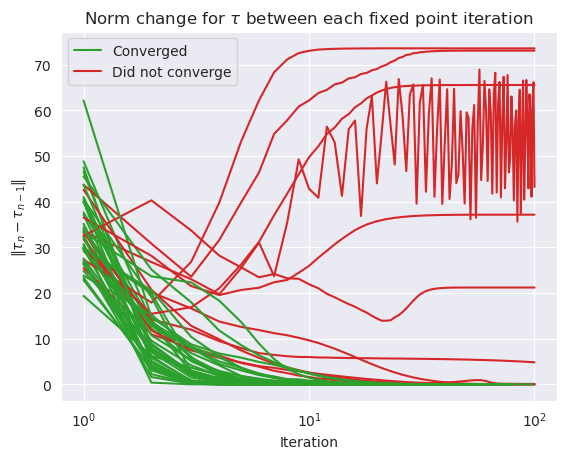
\includegraphics[width=0.8\linewidth]{figures/fixed-point-convergence.png}
        \end{column}
      \end{exampleblock}

    \end{column}
    \separatorcolumn



  \end{columns}
\end{frame}

\end{document}
